
\documentclass[twocolumn]{article}
\usepackage[top=1.1in, left=0.85in, right=0.85in]{geometry}
% \usepackage[utf8]{inputenc}

% \usepackage{supertabular}
\usepackage{amsthm}
% \usepackage{relsize}
\usepackage{amsmath}
\usepackage{amssymb}
% \usepackage{code}
\usepackage{graphicx}
\usepackage{fancyvrb}
\usepackage{url}
\usepackage{textcomp}

\pagestyle{empty}

\newcommand\comment[1]{}

\newcommand\st{$^{\mathrm{st}}$}
\newcommand\nd{$^{\mathrm{nd}}$}
\newcommand\rd{$^{\mathrm{rd}}$}
\renewcommand\th{$^{\mathrm{th}}$}
\newcommand\tm{$^{\mbox{\tiny \textsc{tm}}}$}

% nice fractions
\newcommand\sfrac[2]{{}\,$^{#1}$\!/{}\!$_{#2}$}

\def\signed#1{{\unskip\nobreak\hfil\penalty50
    \hskip2em\hbox{}\nobreak\hfil\sl#1
    \parfillskip=0pt \finalhyphendemerits=0 \par}}

% \newcommand\citef[1]{\addtocounter{footnote}{1}\footnotetext{\cite{#1}}\ensuremath{^{\mbox{\footnotesize [\thefootnote]}}}}

\newcommand\dirham{\protect 
\includegraphics[width=1em]{dirham}}

% \usepackage{ulem}
% go back to italics for emphasis, though
% \normalem

\begin{document} 

% Academic Advancement Advice: Adopt A A Authorship
% Academic Advancement Advice: Author Articles as A A

\title{Academic Advancement Advice: Author Articles as A.~A.}
\author{A.~A. \\
  (tom7.org foundation)
  \thanks{
    Copyright \copyright\ 2018 the Regents of the Wikiplia Foundation.
    Appears in SIGBOVIK 2018 with the abecedarian advantage of the
    Association for Aomputational Aeresy; {\em IEEEEEE!} press,
    Verlag--Verlag volume no.~{\tt std::numeric\_limits<float>::lowest()}.
    1 \dirham
} }

\renewcommand\>{$>$}
\newcommand\<{$<$}

\date{1 April 2018}

\maketitle

\section*{Abstract}
proof at last
    1\ \dirham

\vspace{1em}
{\noindent \small {\bf Keywords}:
  A A A A A A
}

\section{Introduction}

Those with names falling in the dead-middle of the alphabet---like as
a random example, Murphy---have suspected since early life a
disadvantage. For example, when the teacher lines up the students for
pie, in order to be completely fair and avoid bias, orders them by the
perfectly objective criterion of alphabetical order. Occasionally, the
teacher realizes that the same students always get pie first, and
corrects this bias by using {\em reverse} alphabetical order.
Sometimes the teacher uses alphabetical or reverse-alphabetical by
first name, or sometimes last name. All variations of this idea are of
course unfair, as is clear to first- and second-graders, who are
powerless to rebel without (a) status in the K-12 hierarchy (b) the
statistical language in which to formalize their objection and (c)
access to a prestigious conference with permissive publication
standards.

This paper demonstrates that even within academic paper publishing
(which one could argue is obsessed with bias, prestigious conferences,
statistical language for formalizing objections, and status in the
K-12 hierarchy), this unfairness persists. Specifically, we find that
authors whose names come alphabetically earlier have higher citation
rates.

\section{The Data}

I obtained a FISA warrant based solely on a salacious and unverified
memo funded by SIGBOVIK's political opponents. The warrant was for the
AMiner Open Academic Graph~\cite{Tang08ArnetMiner}, which consists of
summary information for 154,771,162 papers in about 130 gigabytes of
JSON data. Then I performed computer science for longer than it should
have taken.


\subsection{Relatable Computer Science Activities}

This subsection contains a relatable tale of computer science. It can
be safely skipped, like all content in this paper.

\smallskip
The task is apparently simple: Parse 130 gigabytes of JSON data to
extract the author names and citations from the papers and count them.
To begin my journey, I selected a C++ JSON library from 39
alternatives listed on a benchmark page.\cite{yip2018native} The first
criterion I ordered by was ``correctness,'' for which only two parsers
achieved the highest correctness score, $100\%$. I selected the slower
(i.e., more methodical) of the two parsers, since I did not want to do
shoddy work.

Next I spent a nice Saturday morning integrating this library into my
private build environment, making sure its open source license was
properly declared and so on, while I waited for the 130 gigabytes of
JSON to download.\footnote{I assure the reader that I have the most
  premium optical-fiber-based Internet. However, the Microsoft Content
  Distribution Network throttled these downloads mightily, presumably
  because of Net Neutrality.} Miraculously, this was straightforward.
I was able to finish writing the code to process the articles before
they even finished downloading. However, upon unzipping, I found that
each file contained one million articles, not as a single JSON array
but as a series of adjacent objects. AdJSONt objects. The JSON library
allowed for reading JSON from files, but {\em not} e.g. for reading a
single record from a file pointer repeatedly. So, I needed to do my
own ad hoc parsing before feeding each record to the JSON library as
strings. OK. Now when I run it, it prints
\begin{verbatim}
  [Segmentation fault
\end{verbatim}

This is not my first segmentation fault---let me tell you!---so I knew
what to do. I debugged the program, adding assertions using a
\verb+CHECK+ macro that aborts if its condition is violated. I
eventually determined that the bug must be inside the JSON library
itself, since the segmentation fault happened between two
\verb+CHECK+s where the only code being run was JSON library code. So,
deciding that perhaps its $100\%$ correctness benchmark score was
overstated, I downloaded and repeated the process with the other,
faster (i.e., more slapdash) parser. Of course this parser has a
different API so I needed to rewrite my program. (The program is very
simple so this was the fastest step; however, getting the library
properly incorporated and compiling and then learning its API still
required me to apply fundamental principles from my advanced computer
science degree.) Once my program was rid of the old crashy library, I
ran it, and it produced this result
\begin{verbatim}
  [Segmentation fault
\end{verbatim}
Since these two libraries produced the same result, either
segmentation violation must be part of the JSON specification, or the
bug is instead elsewhere in the program. After reducing the program to
a fairly simple test case, I determined that it must be some kind of
``Heisenbug'' whereby an earlier piece of code was corrupting the heap
or similar, causing a later crash only when present. This was not my
first Heisenbug---let me tell you!---so I knew what to do. However,
not being able to use Valgrind on Windows (did I mention that I'm
using Cygwin and mingw64 on the eponymous Windows~7 by the way? Why am
I doing that?), I booted Linux in a virtual machine, installed the 87
critical security updates that had been released since I last booted
this virtual machine a few months ago, and compiled my program there.
I then needed to move one of the JSON files to the virtual computer to
test, without having to download 130 GB from the internet again, but
the file was apparently too large to transfer using the mysterious
``Drag and drop to virtual machine'' functionality. I recalled that
VirtualBox can mount a shared folder from the host machine if you edit
the \verb+/etc/fstab+ file to contain the correct code words, and that
I had performed this ritual before, but then had commented-out that
line in ``rescue mode'' because I also learned that having this line
present during the boot process causes a kernel panic. So I
temporarily reinstated the line and mounted the drive and copied the
gigantic file into the virtual machine and then removed the dangerous
magic from the f-stab for f-safety.

Next I ran Valgrind on this minimal test case and it worked as
expected with no unclean behavior detected and no crashing.

Since Linux was no help debugging, I returned to Windows~7 and tried
single-step debugging. Here I discovered that the crash in my minimal
test case was occurring when using \verb+cerr+. Specifically, the
second thing sent to \verb+cerr+ would produce a segmentation fault. I
then recalled that the \verb+CHECK+ macro uses \verb+cerr+ and now saw that
the \verb+[+ in \verb+[Segmentation fault+ was probative, for this
was the location of the original crash:
\begin{Verbatim}[fontsize=\small]
    std::cerr << "[" << pretty_date_.HumanDate() << "] "
              << file << ":" << line << ": ";
\end{Verbatim}

Of course, inside \verb+HumanDate()+ I found a hasty patch I had
installed in A.D.~2014 called ``make logging not spit garbage on
mingw,'' suggesting that I had encountered and misdiagnosed this issue
in the past. Although this led me on a minor herring (e.g. is
\verb+__MINGW32__+ defined when cross-compiling for x86\_64?)
HumanDate just returned \verb+"mingw"+, so this really was a problem
with \verb+std::cerr+ crashing on the second thing printed with it
(i.e., with the returned \verb+ostream+).

Minimizing the test case, this bug only occurred after reading a large
file all in one syscall (for ``performance'', even though doing these
huge reads basically locks up my machine). Specifically the file was
2,105,319,548 bytes, which is $98\%$ of $2^{31}$, suggesting the
possibility of integer overflow in some buffer-sizing code in the
weird Cygwin or mingw wrappers for \verb+fread+, \verb+fstat+, etc.
This could plausibly cause corruption of the \verb+cerr+ ostream,
which is probably part of the same code.

Preparing to at least make a bug report if not try to fix it, I
upgraded my compiler and runtime from GCC version 5.1.0 to 6.4.0,
and the problem completely went away. Since Valgrind also agreed
that there was no issue, I chalked this one up to simply an internal
C runtime bug that someone else found and fixed in the last 2 years.
Thanks!

With \verb+cerr+ fixed, I could now easily see the original ``bug'',
which was a violated assumption: I expected (and \verb+CHECK+ed),
optimistically, that if the article had an {\tt author} field then the
author would be a string. I accounted for a missing author, an author
that was the empty string, but not {\tt author: null}. Thanks!

Finally, I could run the author and citation tallier on all of the
JSON files. However, two of the files appeared to be empty. Although
this was only a small percentage of the articles, I did not want to
skip any because it's possible that they are arranged in a non-random
order (e.g. alphabetically!) and that this would bias the results. I
learned that although the AMiner database is helpfully split into
files each containing one million articles, for ease of handling, two
of these files are nonetheless slightly larger than $2^{31}$ bytes. Such
files cannot be cleanly sized with \verb+fstat+ (the \verb+st_size+
field has type \verb+off_t+, a signed 32-bit type in POSIX) and even
if you follow the standard advice of just treating it as unsigned
anyway, \verb+fread+ will simply fail when asked to read such a large
chunk\footnote{
%
  Curious why I am even using {\tt fstat} and {\tt fread} like some
  dramatically bearded guy from the 1980s? I have my own library
  routine for reading a file into a string. When working with large
  files it's useful to avoid copying, because the contents of the file
  may be a significant fraction of all RAM---copying is not only
  expensive, but might temporarily exceed the available RAM. So, you
  need to allocate the buffer ahead of time and avoid resizing it
  (which often also performs a copy). It seems like something that
  everyone would want to do, but it's ridiculously hard to do portably
  in C or C++. Specifically, there seems to be no way to actually know
  the size of a file so that you can size the buffer ahead of time.
  For example, {\tt fseek} to {\tt SEEK\_END} and {\tt ftell} does
  {\em not} work (it has {\em undefined behavior}). The {\tt st\_size}
  field from {\tt stat} also does not give correct results e.g. when
  reading from the {\tt /proc} filesystem. My routine attempts to
  guess the size of the file and perform a single read in the case
  that the guess is correct, while still usually avoiding copying or
  needless work in the case that it's an under- or over-estimate.
%
} despite the fact that it takes \verb+size_t+, an unsigned type. (?!)
So, another afternoon spent doing Computer Science. But all you need
to do of course is perform multiple sequential reads.

Finally, the trivial task of counting the number of articles and
citations per author could be completed.

\section{The Data}

This citation database is very noisy. About $1.6\%$ of articles have
no authors, and another $1\%$ have a blank (or {\tt null}) author. I
verified the comprehensiveness of the dataset by finding my own author
record(s)\footnote{This paper is published under the pseudonym A.~A.,
  standing for Awesome Author, obviously in order to increase its
  citation rate. Normally I publish as Tom Murphy VII, which can be
  found in citations with many broken variations, such as ``Vii, T.''}
and 275 citations ({\bf Yeah!!}). I also spot-checked that the database
includes prestigious conferences, which it does, at least including
the ``article'' {\em A Record of the Proceedings of SIGBOVIK 2008},
with author {\em Pennsylvania USA}. It was necessary to normalize
author names to remove punctuation, weird unicode stuff like non-breaking
spaces, javascript-encoded newlines and nul-bytes, and so on. There
are many strange authors in the database, such as
\begin{itemize}
\item capinha para celular horizonte artificial iphone \quad(no citations)
\item +0aaaaaabablaaaaaea\&\#xa \quad(no citations)
\item a h poop \quad(4 citations)
\item john mcm anus\footnote{Presumably a hostile citation of John McManus.} \quad(2 citations)
\item coffee hour \quad(0 citations)
\item nominate com registering dad domains since \quad(0 citations)
\item a a \quad(195 citations)
\item a a a a m islam \quad(6 citations)
\end{itemize}

On the other hand, from this hand-picked sample we can already see the
citation advantage of having a name that's alphabetically early. Some
authors seem to have already intuited this fact.

\section{Author Analysis} \label{sec:authoranalysis}

Author names appear in both ``Firstname Lastname'' order and
``Lastname Firstname'' (when this grammar is even applicable).
Therefore, I analyzed alphabetizing from front to back (by
space-separated token) as well as back to front. I also rejected a
large number entries when I could not place the name in alphabetical
order because its first character was not ASCII. Later non-ASCII
characters are OK, and are just sorted by their UTF-8 encodings (or
whatever garbage is in the file). This of course produces a bias
(excluding authors who write their names in e.g. Cyrillic and CJK
scripts), although it's not clear how to assess the alphabetical
hypothesis for them.

To visualize the data, I produced a cumulative distribution function
(CDF) for both articles and citations. Considering each author in
alphabetical order, I keep a running total of how many articles and
how many citations have been seen so far. The x-coordinate is the rank
of the author (its index in the alphabetical list) and the
y-coordinates are the fraction of articles (or citations) seen so far.
The CDFs for the forward and backward token orders are in
Figure~\ref{fig:authorcdf}.

\begin{figure*}[t]
  \begin{center}
  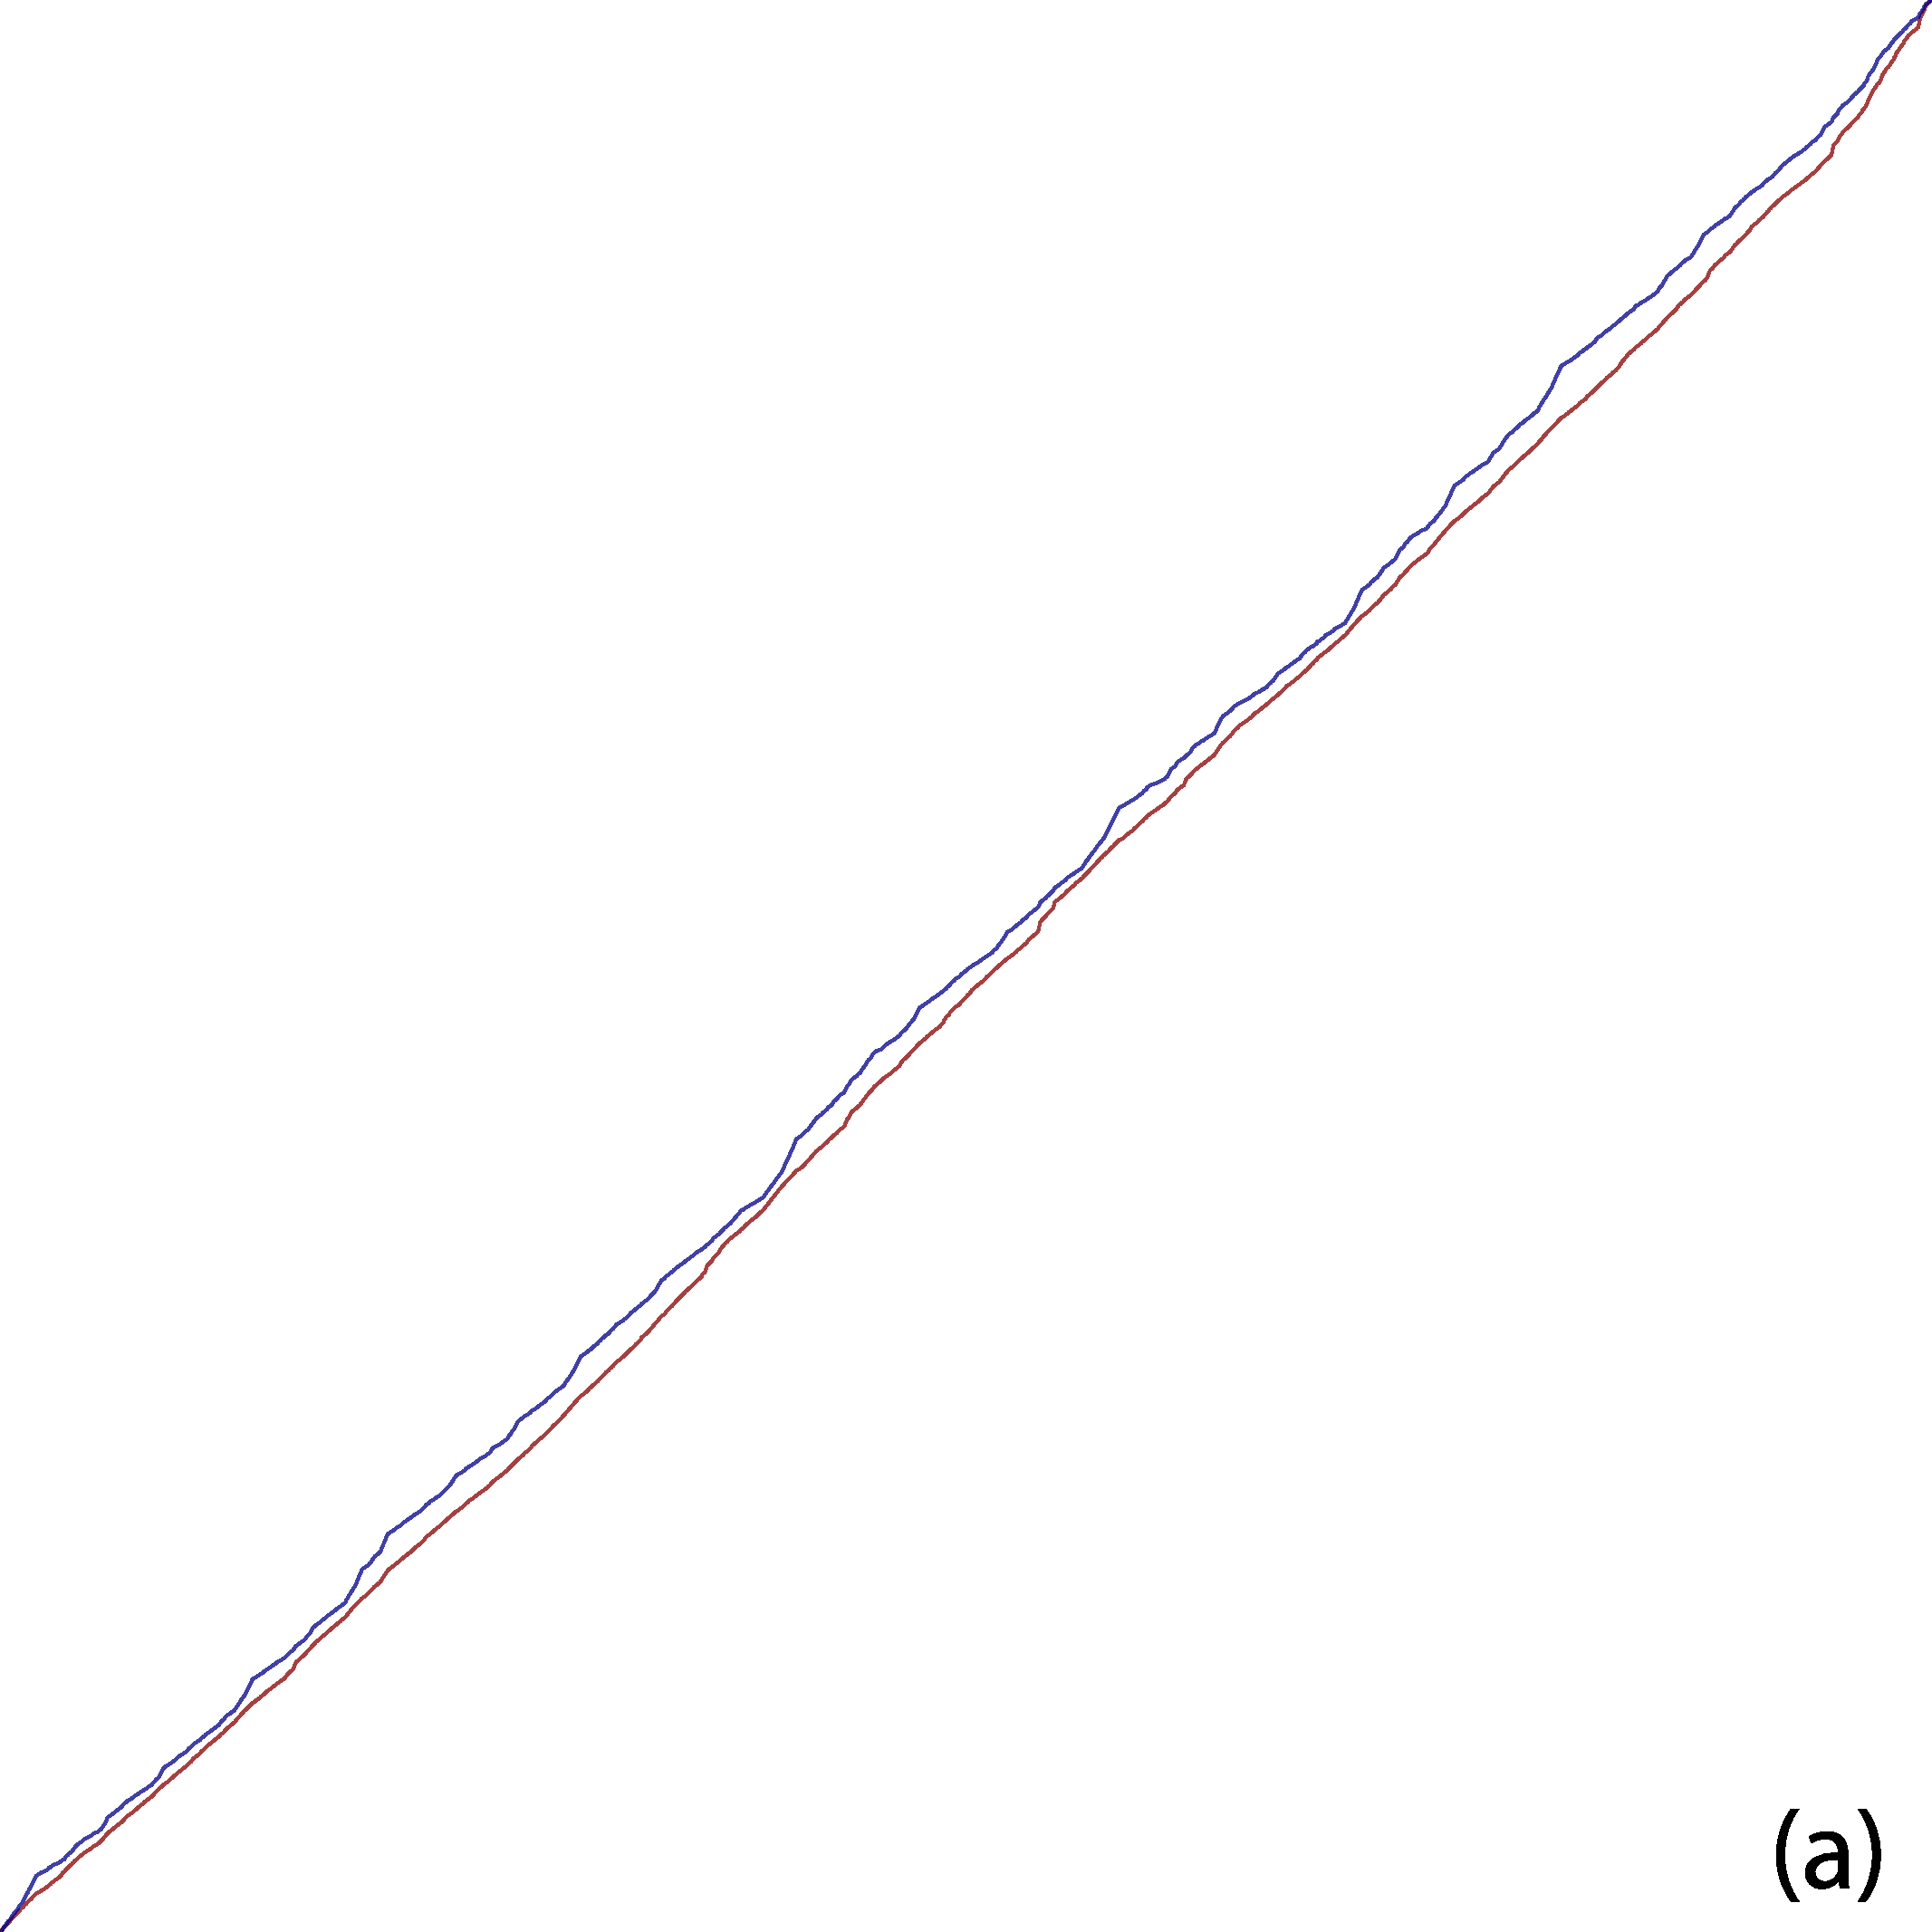
\includegraphics[width=0.44 \textwidth]{authorstats-forward}
  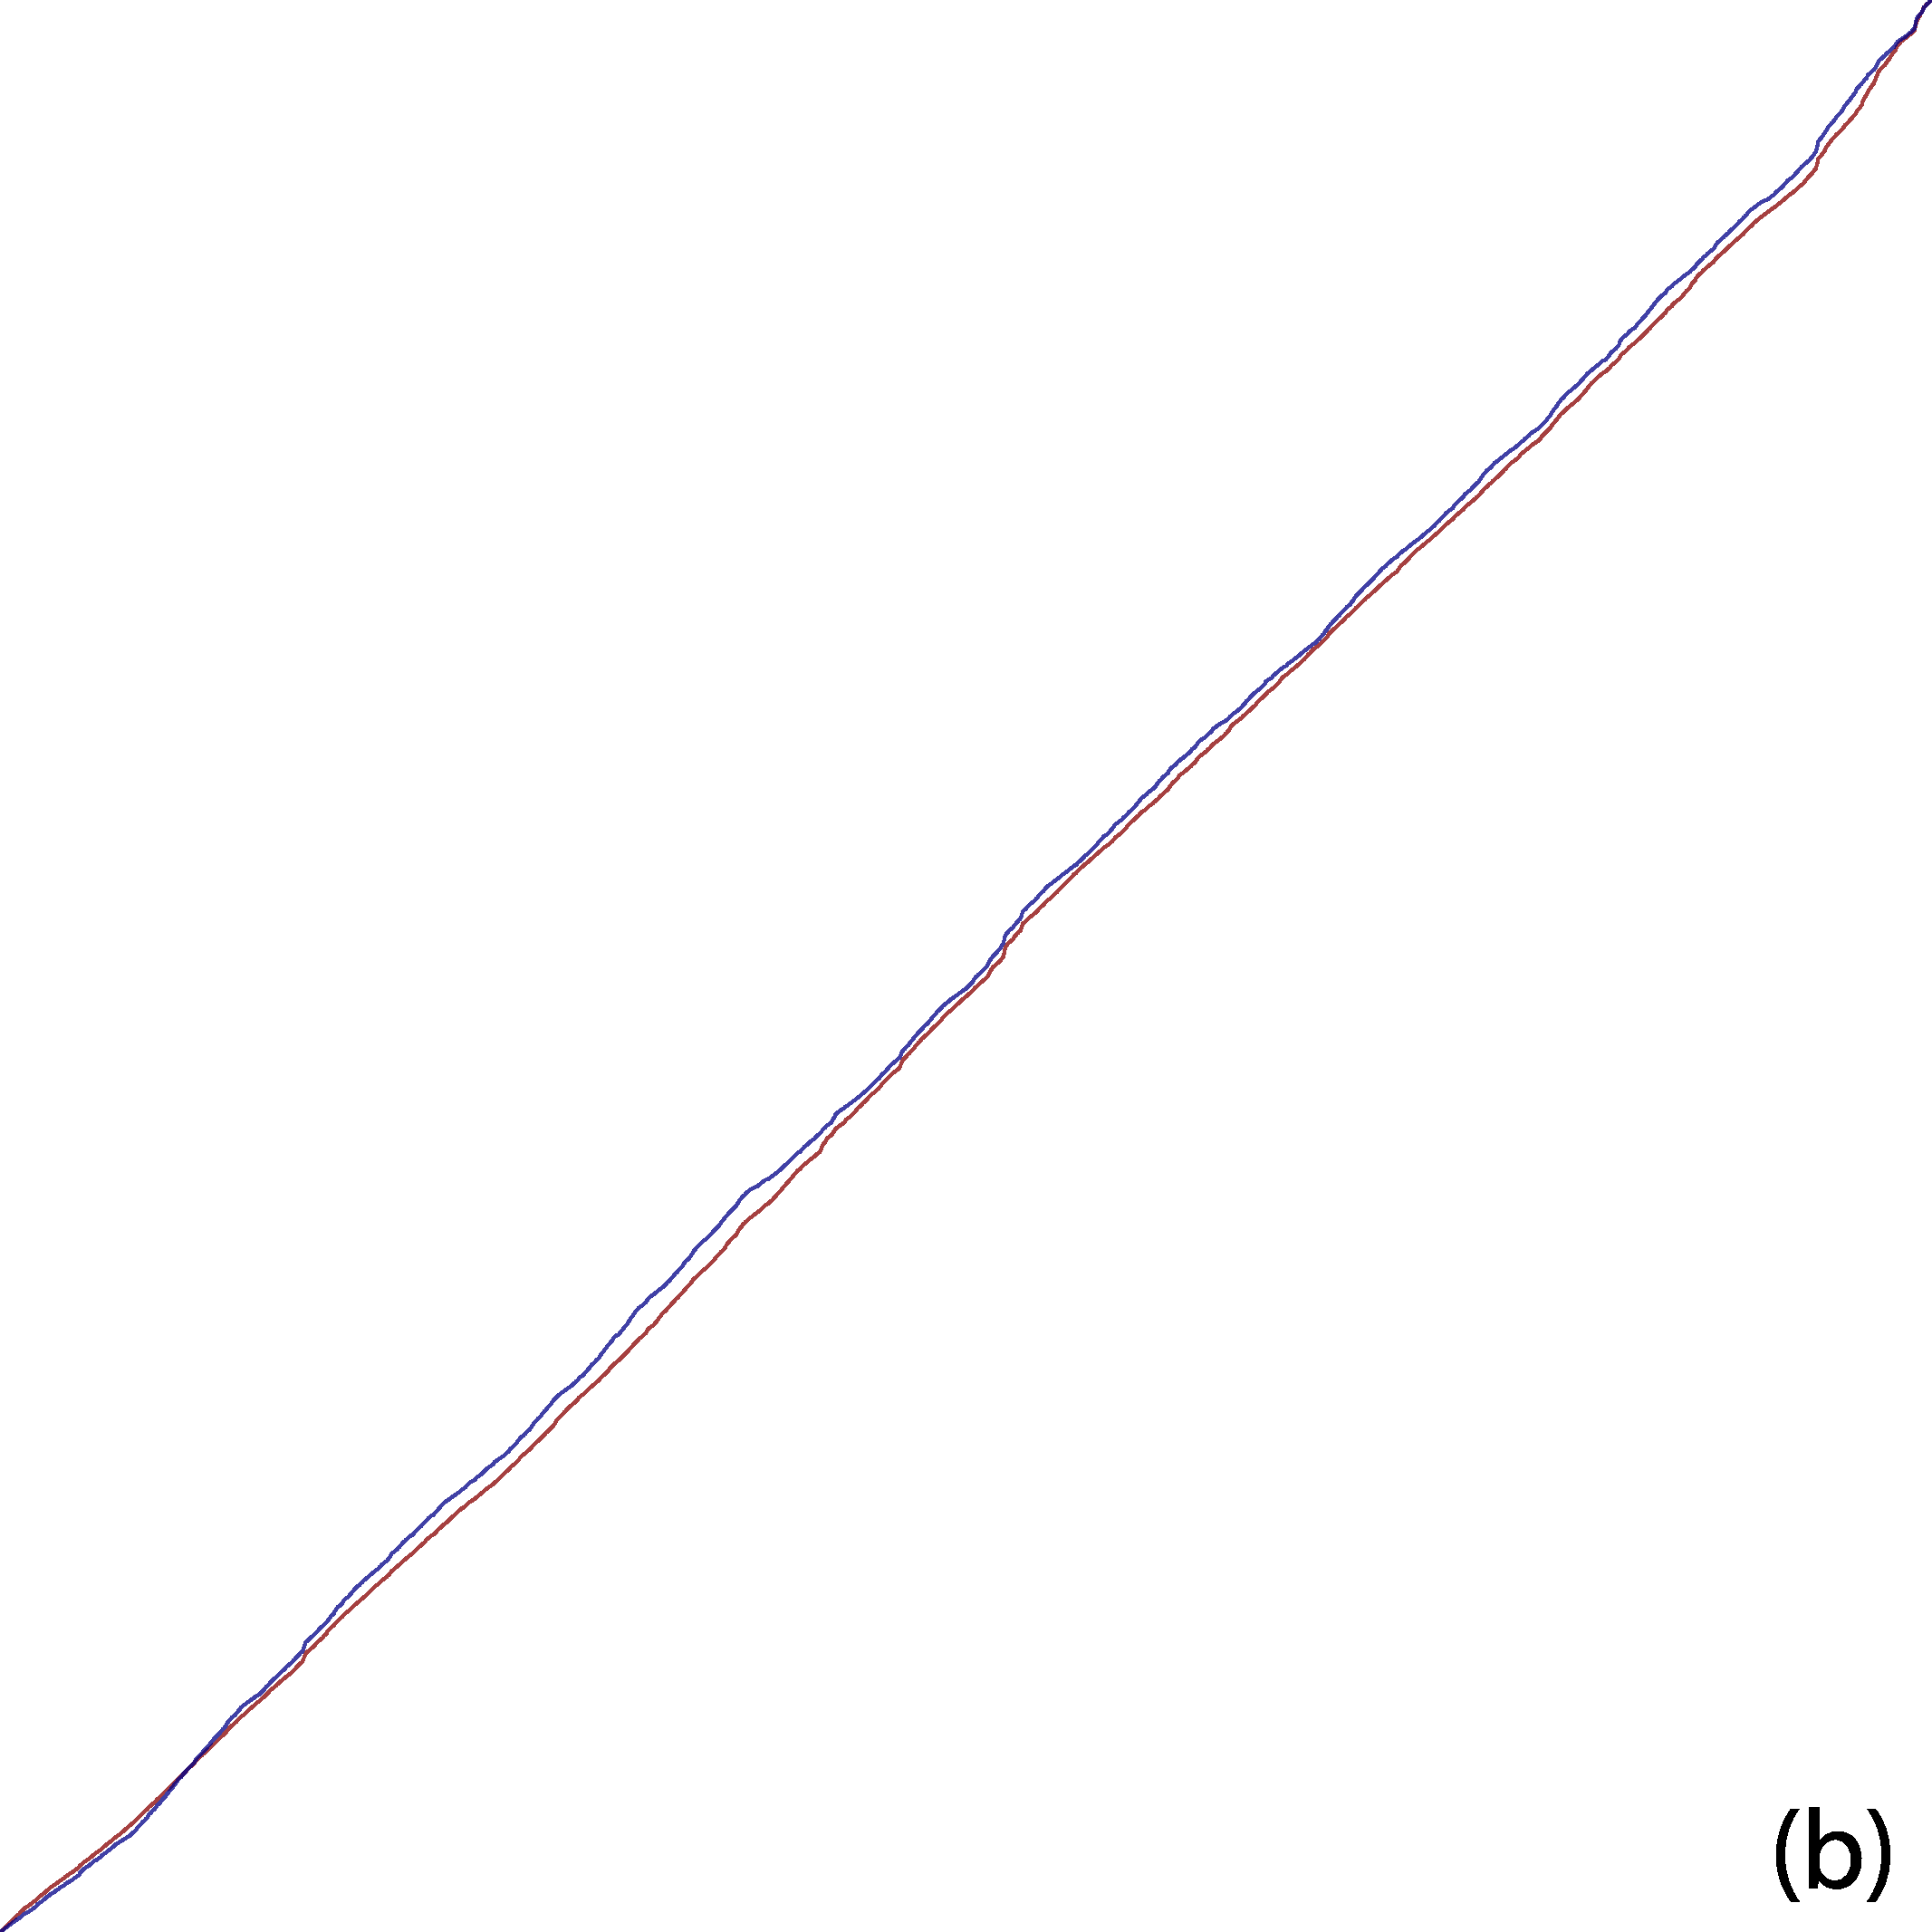
\includegraphics[width=0.44 \textwidth]{authorstats-backward}
  \end{center}
  \caption{ Author CDFs for (a) forward token order and (b) backward
    token order. (For example, (a) treats {\tt tom murphy vii} as
    coming between {\tt tom marphy} and {\tt tom myrphie vxx} and (b)
    treats it as coming between {\tt zzz murphx vii} and {\tt a
      viii}.) The x-axis is the author's position alphabetically among
    all authors. The blue lines are the fraction of all citations seen
    so far, and the red lines the same for articles. The lines must
    meet at $(0,0)$ and $(1,1)$ by definition. When the blue line is
    above the red, the number of citations is outpacing the number of
    articles for authors alphabetically before this point. Since you
    may be reading in old timey blacke \& whyte, I will also tell you
    that the blue line is more or less above the red line in both
    pictures. This means that both show a bias towards the early
    alphabet, with the forward direction being more dramatic (for
    basically the entire range). The backward range briefly shows the
    opposite bias (crossing over at author \#5,400,000, ``ojars
    biskaps''), suggesting that the best names may be alphabetically
    early but in the {\em B}s, not {\em A}s. The poorer performance of
    A-names may be due to authors attempting to ``game the system'' by
    publishing with names like ``a a.'' } \label{fig:authorcdf}
\end{figure*}

These CDFs show that---as expected!---there is a bias towards citing
authors alphabetically early, whether we order alphabetically by
``first name'' or ``last name.''

There are multiple hypothesized causes:
\begin{itemize}

\item When writing a last-minute ``related work'' section, authors
  sometimes find papers to cite in alphabetical order, for example, by
  reading another paper's bibliography, which is sometimes
  alphabetized.

\item Sometimes the last page of a manuscript is ``lost,'' truncating
  its alphabetical bibliography to some prefix.

\item Some academics try to \verb+fread+ all papers into memory, but
  it fails on the file that's just slightly larger than $2^{31}$ bytes,
  and so the papers therein don't get cited, and those papers are
  alphabetically in the middle or end of the alphabet.

\item When applying for grad school, tenure track faculty jobs, grants,
  and so on, packets are alphabetized ``for fairness,'' and the
  mood of the committee becomes more irritable as they make
  progress through the set.

\item Decreased access to pie and exposure to unfair situations in
  youth cause a lifelong predisposition to failure.

\end{itemize}

\section{I now bore of the titular topic. Let us discuss new topics.}

Specifically, let's discuss titles. Some have suggested that the
titles of papers also affect their citation rates, and it is
reasonable to suspect that an alphabetical bias could apply here as
well. After applying some light normalization, I extracted each of the
words that appear in the titles of all papers, counting both the
articles (an article is only counted once per word, even if that word
appears multiple times in its title) and citations. This tells us
what the expected number of citations for an article is (assuming
independence, which is---as usual---completely false) when its
title contains a word. Considering only words that appeared in
at least 100 articles, here are the top by expectation:

\begin{tabular}{l|l|l|l}
{\bf word} & {\bf articles} & {\bf citations} & {\bf E = c/a} \\
  \hline
folin & 172 & 209,642 & 1,211.8 \\
power/knowledge & 111 & 55,992 & 499.9 \\
\{s\} & 101 & 38,241 & 374.9 \\
1972-1977 & 171 & 54,917 & 319.2 \\
\textbackslash sqrt\{s\} & 126 & 33,253 & 261.8 \\
eigenfaces & 176 & 45,284 & 255.8 \\
america''s & 119 & 30,478 & 253.9 \\
gromacs & 125 & 30,865 & 244.9 \\
neo-ffi & 102 & 21,992 & 213.5 \\
esh & 156 & 33,142 & 211.1 \\
\end{tabular}

These are mostly explained by being relatively rare words that appear
in extremely popular papers. For example, {\em folin} comes from an
1951 paper\cite{lowry1951protein} describing a procedure for using
this reagent, which I guess everyone who uses this technique cites
(Google scholar has this paper at 215,329 citations). {\em
  Power/knowledge} and {\em 1972-1977} both come from the title of a
Foucault book\cite{foucault1980power} with 31,590 citations.

Considering just the alphabetizable words, these too show a bias
towards early words (Figure~\ref{fig:wordcdf}). Bibliographies that
are alphabetized by title could exhibit the same effects discussed in
Section~\ref{sec:authoranalysis}. Additionally, since some scholars
learn English by reading the dictionary front to back, they may
simply be more practiced at early words and find them more attractive
or easier to understand.

\medskip
It is a bit easier to interpret the expected citation numbers if we
normalize them. The average citation rate of all articles in this set
is 5.1261. This may seem high, especially considering the 90 million
articles with no citations, but keep in mind that most papers have
bibliographies in which they cite several others. Data quality issues
aside, this is basically the same as saying that the averge
bibliography length is 5.1261. We can assign each word a ``citation
multiplier'' effect now, defined as simply
$$
\mathrm{multiplier}_w = \frac{\mathrm{citations}_w / \mathrm{articles}_w}{5.1261}
$$
and now numbers greater than 1 improve your chances at citation, and
numbers less than 1 diminish it. Here are the most common words:

\begin{tabular}{l|l|l|l}
\,  & artices & citations & multiplier \\
  \hline
of & 64322278 & 366756237 & 1.207822 \\
and & 42576889 & 276526184 & 1.375780 \\
in & 39685539 & 230534759 & 1.230526 \\
the & 38873614 & 216491707 & 1.179704 \\
a   & 22666824 & 139244700 & 1.301292 \\
for & 19048050 & 114197875 & 1.269972 \\
on & 15194275 & 68904896 & 0.960631 \\
with & 10825547 & 60752792 & 1.188784 \\
to & 10202749 & 58590695 & 1.216461 \\
de & 7753205 & 3283786 & 0.089718 \\
by & 7259598 & 42234470 & 1.232370 \\
from & 5389957 & 35999433 & 1.414806 \\
an & 5368923 & 33088995 & 1.305519 \\
la & 4417389 & 1471023 & 0.070541 \\
study & 4370395 & 22022172 & 1.067397 \\
\end{tabular}

Several of these words are visible in Figure~\ref{fig:wordcdf}, in
fact; they are so common that they cause large jumps in both article
and citation count. Curiously, most of the common words have a
multiplier greater than 1; they {\em increase} the expected number of
citations. {\em of} sounds smart (e.g. {\em Of Mice And Men}), {\em
  and} makes sense (paper contains at least two results). On the other
hand, {\em on} actually reduces the citation count, probably because
it implies equivocation (e.g. {\em On the other hand}). Dramatically,
common non-English words have very low multipliers; Spanish words {\em
  de} and {\em la} reduce citations by a factor of more than ten. This
may be due to problems in the data set, but it is certainly easy to
imagine real cultural bias!

Finally, here are the words with the worst multipliers:
\begin{tabular}{l|l|l|l}
313779.  
\includegraphics[width=2em]{bookreview} & 29582 & 1 & 0.000068 \\
313778.  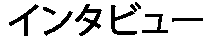
\includegraphics[width=5em]{interview} & 20547 & 1 & 0.000097 \\
313777.  facharzt & 85315 & 9 & 0.000117 \\
313776.  f3d & 125257 & 15 & 0.000128 \\
313775.  recenzja & 63568 & 8 & 0.000142 \\
313774.  newhaven & 13296 & 1 & 0.000150 \\
313773.  secr\'etaire & 12267 & 1 & 0.000163 \\
313772.  zahnarzt & 17958 & 2 & 0.000167 \\
313771.  libguides & 389727 & 72 & 0.000187 \\
313770.  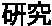
\includegraphics[width=2em]{research} & 12961 & 2 & 0.000231 \\
313769.  
\includegraphics[width=1em]{that} & 15984 & 3 & 0.000250 \\
313768.  kitas & 7713 & 1 & 0.000259 \\
% 313767.  シンポジウム & 18539 & 4 & 0.000270 \\
% 313766.  特集 & 878011 & 240 & 0.000274 \\
\end{tabular}

For this set, I only considered words that appeared in the title of at
least one paper that was actually cited. The worst multiplier is

\includegraphics[width=2em]{bookreview}, which is Chinese for ``book
review;'' it reduces your chances of citation by more than ten
thousandfold. Close by is 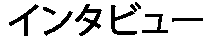
\includegraphics[width=5em]{interview},
Japanese for ``interview.'' {\em Facharzt} is like (medical)
``specialist'' in German, {\em recenzja} is ``review'' in Polish, and
{\em newhaven} is a misspelling of a city in Connecticut where I grew
up and was unfairly and repeatedly placed in the middle of lines. But
most of these are just generic non-English words
(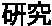
\includegraphics[width=2em]{research} is Chinese for ``research'' and

\includegraphics[width=1em]{that} Korean for ``that'').

\begin{figure}
  \begin{center}
  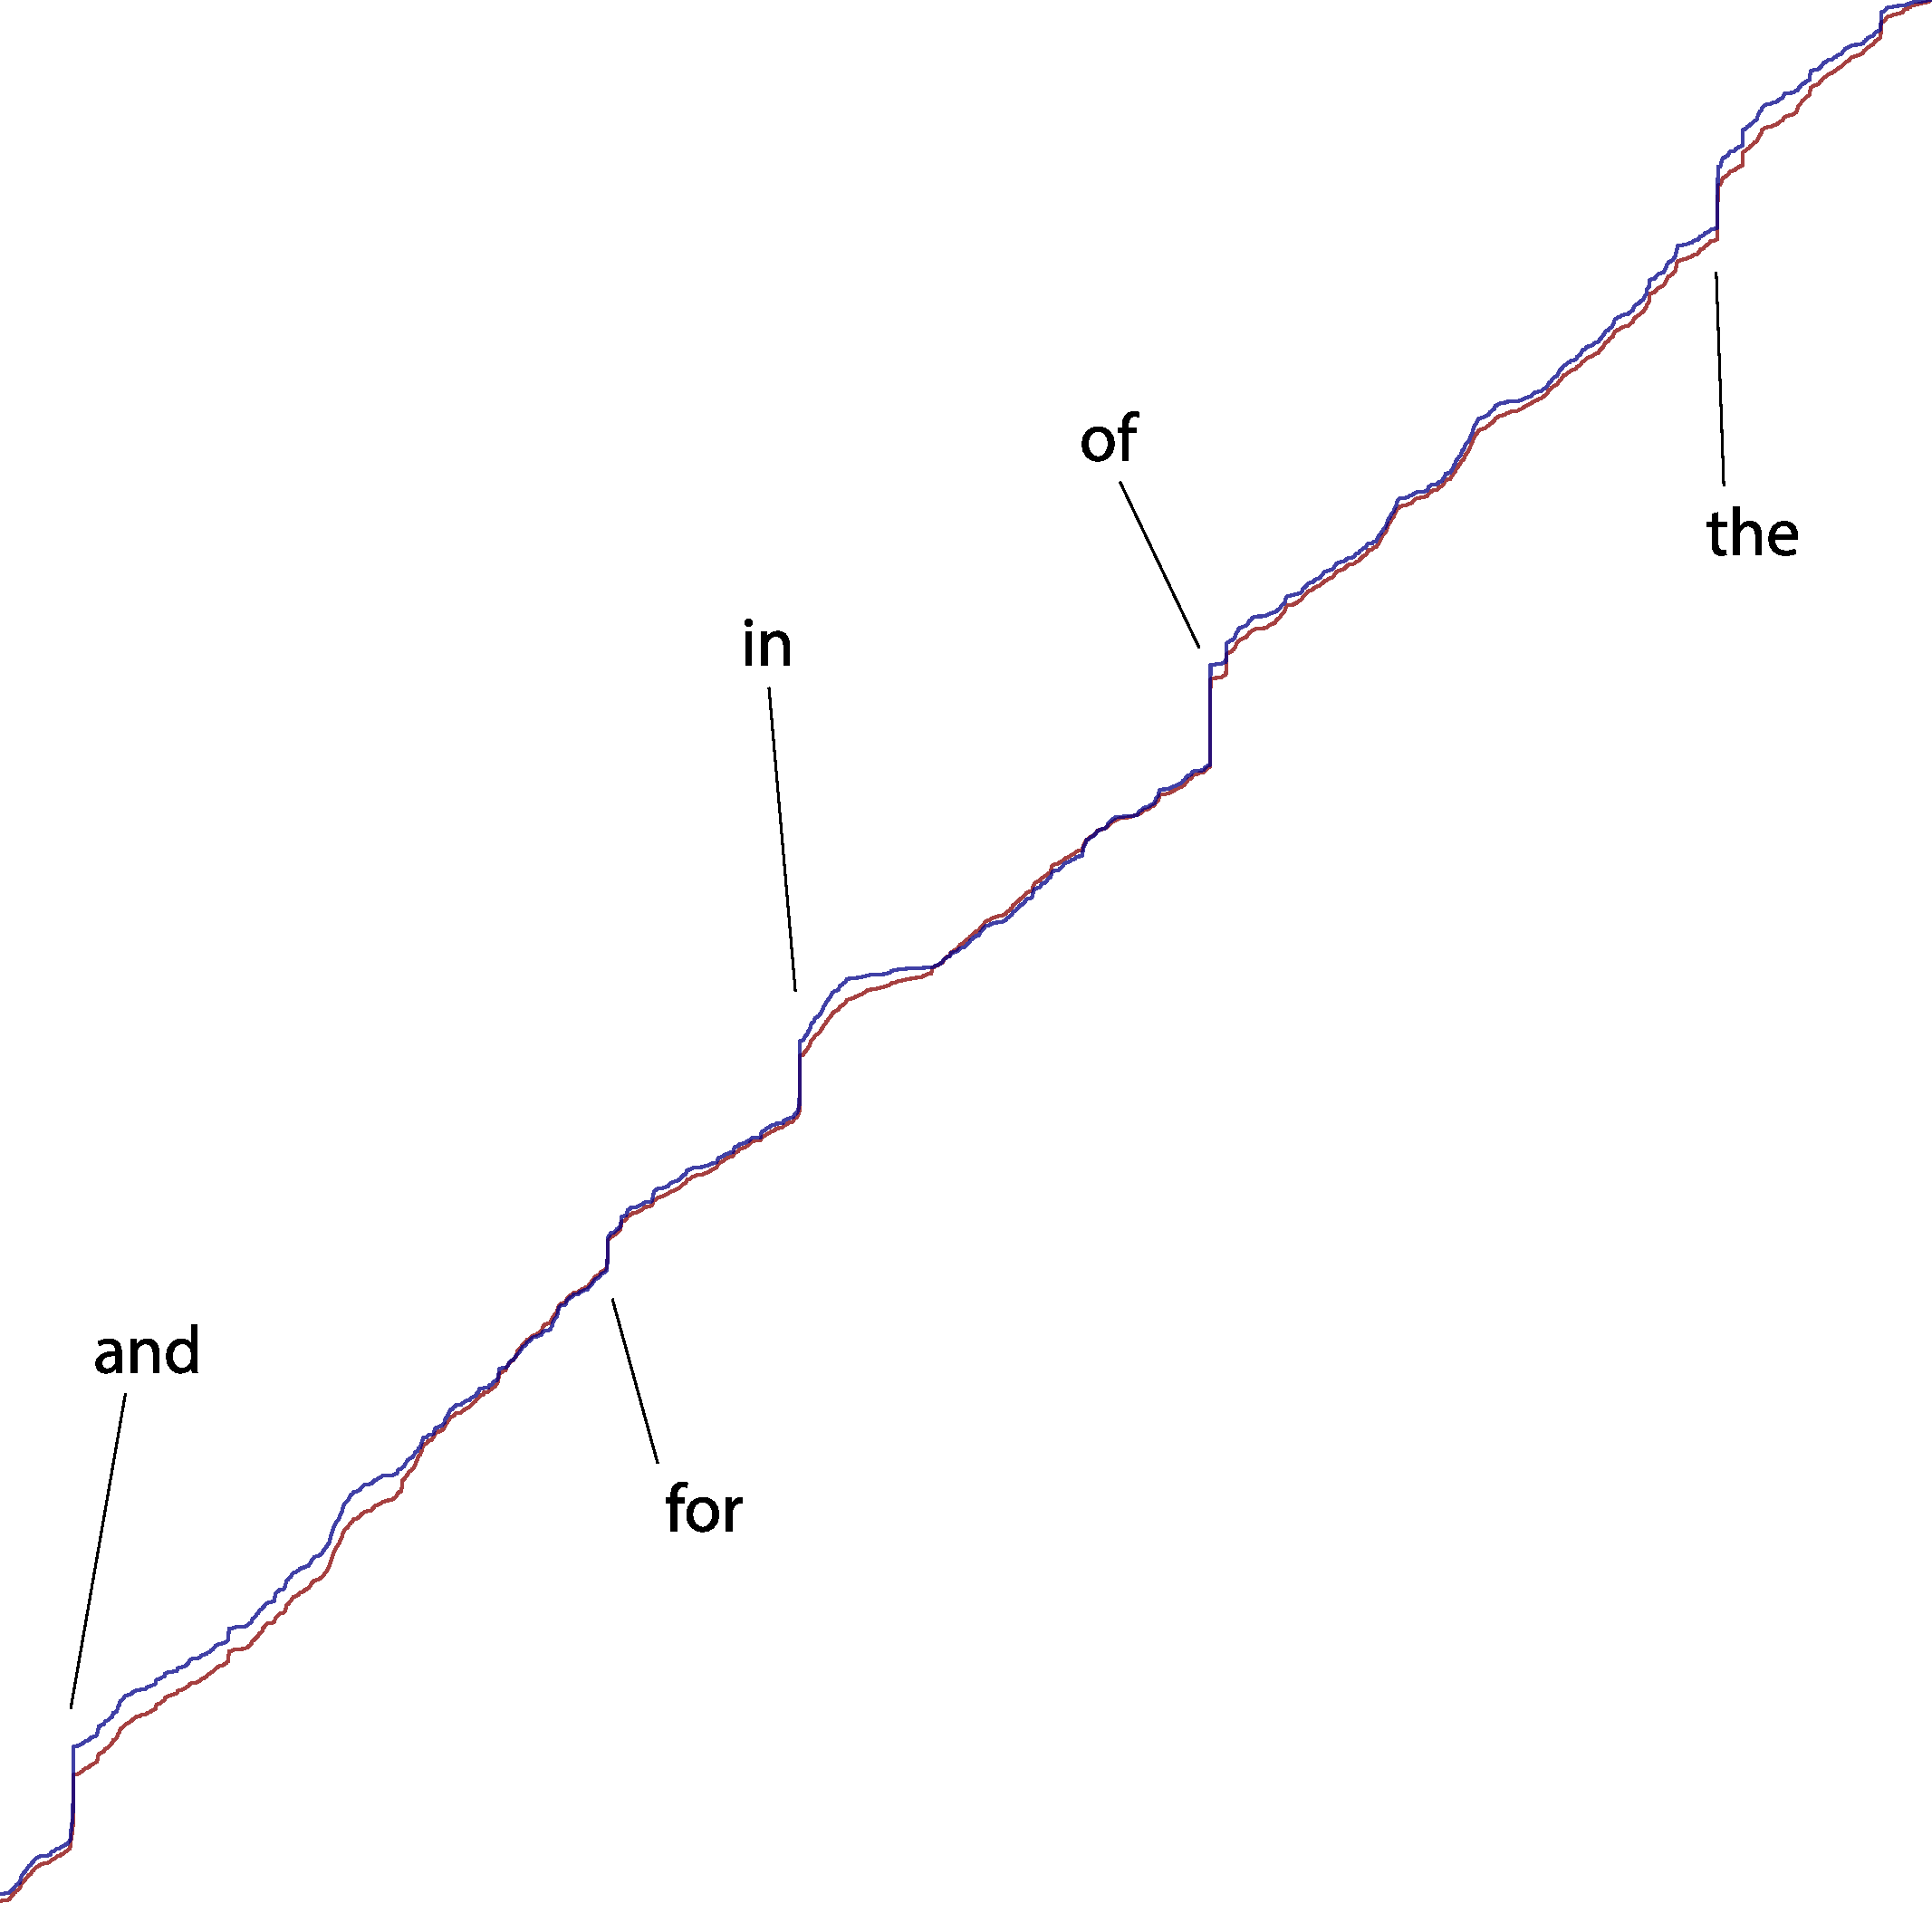
\includegraphics[width=0.475 \textwidth]{wordstats}
  \end{center}
  \caption{ CDF for words arranged alphabetically. This is just as
    in Figure~\ref{fig:authorcdf}, but since each entry is a single
    word, there is no need to treat forward and backward differently.
    Again, we see a small alphabetical bias, with citations leading
    articles for most of the range. In fact, papers that include the
    very first word, ``a'', are cited $1.3\times$ as often as the
    average paper. Other common and advantageous words are visible
    as clear bumps.
  } \label{fig:wordcdf}
\end{figure}

\section{What is the least citable paper?}

Thinking about first and last, one could reasonably ask: Of all
papers, what are the least citable ones? Of course, the paper should
have never actually been cited, but in the database there at least 90
million articles with no citations, all tied for this distinction. Can
we rank among these papers to break the tie?

(Of course I am just poking fun, not seriously declaring these
articles somehow ``worst.'' Many good articles are never cited. For
example, as far as I know, the paper you are reading right now has no
citations.)

One way to do this is to try to estimate the number of citations that
a paper will get based on the words in its title. Since we already
collected the words that are most citable, this is an apparently
simple affair. We can estimate the citation rate by just taking the
product of the multipliers for the words. We treat words for which
we don't have data (because they didn't meet thresholds) as having
multiplier 1.

This first cut has some problems. As an illustration, the article
with the highest estimated citation rate (among those with zero actual
citations) is a paper\cite{leigland2009grid} called
\begin{quote}
Grid Grid Grid Grid Grid Grid Grid Grid Grid Grid Grid Grid Grid Grid Grid Grid Grid Grid Grid Grid Grid Grid Grid Grid Grid Grid Grid Grid Grid Grid Grid Grid Grid Grid Grid Grid Grid Grid Grid Grid Grid Grid Grid Grid Grid Grid Grid Grid Grid Grid Grid Grid Grid Grid Grid Grid Grid Grid Grid Grid Grid Grid Grid Grid Grid Grid Grid Grid Grid Grid Grid Grid Grid Grid Grid Grid Grid Grid Grid Grid Grid Grid Grid Grid Grid Grid Grid Grid Grid Grid Grid Grid Grid Grid Grid Grid Grid Grid Grid Grid Grid Grid Grid Grid Grid Grid Grid Grid Grid Grid Grid Grid Grid Grid Grid Grid Grid Grid Grid Grid Grid
\end{quote}
which is expected to have 5,262,751,498,750,000,000,000,000 citations.
This is because the word {\em grid} has a favorable multiplier and is
repeated 121 times. 

So I limited it to articles with no more than 20 words in the title
(arbitrary). Now the least citable articles all look like this:

\begin{quote}
  IMPLEMENTASI PERATURAN MAHKAMAH AGUNG NOMOR 1 TAHUN 2008 TENTANG
  PROSEDUR MEDIASI DI PENGADILAN (STUDI PUTUSAN MEDIASI DI PENGADILAN
  NEGERI SAMARINDA)\footnote{Translated: IMPLEMENTATION OF REGULATION
    OF THE SUPREME COURTS NUMBER 1 OF 2008 ABOUT MEDIATION
    PROCEDURES IN THE COURT (STUDY OF DECISION MEDIATION IN THE COURT
    SAMARINDA COUNTRY)}
\end{quote}

Which appears to be a real dissertation\cite{putri2009implementasi}
(bachelor's degree of law) from a student in Indonesia, but there are
literally thousands of similar looking papers. Given its company, it
may very well be truly the least citable paper, or it may be a systematic
data problem, or even spam. But I was hoping for some English language
articles so that we could appreciate the joke together in the native
tongue. 

Even filtering for articles with \verb+"lang"+ explicitly set to
\verb+"en"+, I needed to manually create a blacklist of hundreds of
non-English words that commonly appeared in these article titles.
After a few rounds of blacklisting, some ``English'' articles started
to appear:

\begin{quote}
 Office Hours: Monday, Wednesday, Thursday and Friday 9:00 a.m. to 5:00 p.m.; Tuesday 9:00 a.m. to 6:45 p.m \\
  \signed{(citation multiplier $5.37\!\times\!10^{-27}$)}
\end{quote}

\begin{quote}
	Thomas Aquinas: Theologian By Thomas F. O'Meara, O.P. Notre Dame, University of Notre Dame Press, 1997. 302 pp. \$16.95 \\
  \signed{(citation multiplier $6.05\!\times\!10^{-27}$)}
\end{quote}

The first is probably not the title of an article\cite{officehours},
although we can agree that it is unlikely to be cited. The second is
probably a bad entry, with the entire citation packed into the title
field. This book actually does have 94 citations (or DOES
IT?~\cite{o1997thomas}) on Google Scholar and an Amazon Sales Rank of
\#10,837 in {\em Christian Denominations \& Sects}.\footnote{ On the
  other hand, the entry does have a different
  author\cite{stevenson2000thomas}, so it could possibly be a review
  of this book whose title is literally the string above, including
  the price?} In order to prevent such data problems from affecting
our results, I then added a requirement that the article have basic
metadata (either a Digital DOI Identifier field or {\tt venue}) for it
to be considered. There are still many broken entries, but picking through
the results I'm able to find what appear to be actual articles:

\begin{quote}
  % 48654527.  5.8084026066881388e-026	56d918ecdabfae2eee6c6965
  Eight contemporary poets : Charles Tomlinson, Donald Davie, R.S. Thomas, Philip Larkin, Ted Hughes, Thomas Kinsella, Stevie Smith, W.S. Graham
  \signed{(citation multiplier $5.8\!\times\!10^{-26}$)}
\end{quote}

% 48654111.  1.7552310525171227e-019	53e99952b7602d9702190ac1	The 80th Birthday of Sir Henry Dale, O.M., G.B.E., M.D., F.R.C.P., F.R.S.: Salute to Henry Hallett Dale

% 48654054.  2.7492425189773547e-019	56d8ecc5dabfae2eee5b30f5	Narratives Unsettled: Digression in Robert Walser, Thomas Bernhard, and Adalbert Stifter by Samuel Frederick (review)

% 48552586.  5.0644175742872403e-019	56d9266ddabfae2eeebdd19a	Catherine Mowry LaCugna's Trinitarian Theology: III- The Ecumenical Implications of Catherine Mowry Lacugna's Trinitarian Theology

% 48552476.  1.7011818225031437e-018	56d85cd0dabfae2eee5cb5f4	Texts Illustrating the Causality of the Sacraments from William of Melitona, Assisi Bibl. Comm. 182, and Brussels Bibl. Royale 1542

% 48552391.  3.4094058998675013e-018	53e9bce1b7602d9704965e64	Shakespeare's Titus Andronicus and Bandello's Novelle as Sources for the Munera Episode in Spenser's Faerie Queene, Book 5, Canto 2

Lessons learned:
The least-cited works take the following typical forms. Acade
1. memorials for dead guys
2. reviews of books
3. articles not in english
4. broken citations

\medskip
Of course, since these papers are all notable for being so extremely
uncitable, the true least citable papers are the next least citable,
according to this analysis.

% Tourney -- what is wrong here?
%  1000.000 Mrounds:
%  (69.66 vs. 72.69 Gcit) (6.72 vs. 7.20 Gart) (0.281 vs. 0.295 Gwin)
%  (0.958361 L:R cit) (0.933736 L:R art) (0.280867 vs. 0.295327 win rate)

\subsection{Alliterative Articles}

Adopting an all-'A' affect also advances articles. Although affairs
are abbreviated, adequate abstracts abound: Astronomy, asthma,
atmospheric acclimatization, autobiography, Azerbaijani accents,
acceleration, and abundant alternatives. After achieving academic
accomplishments, acknowledge A.A.'s {\it Academic Advancement Advice:
  Author Articles as A.~A}!

% arranged alphabetically.

strange authors:

u fucks
a a fucks

\begin{verbatim}  
{"id": "56d8981adabfae2eee20314b", "title": "IMPLEMENTASI PERATURAN MAHKAMAH AGUNG NOMOR 1 TAHUN 2008 TENTANG PROSEDUR MEDIASI DI PENGADILAN (STUDI PUTUSAN MEDIASI DI PENGADILAN NEGERI SAMARINDA)", "authors": [{"name": "frianur ivan zairani lisi insan tajali nur"}], "year": 2013, "lang": "en"}
{"id": "56d8a690dabfae2eee9057b0", "title": "Pengaruh Pengawasan Inspektorat Dan Partisipasi Dalam Penyusunan Anggaran Terhadap Kinerja Manajerial SKPD (Studi Empiris Pada Instansi Pemerintah Kabupaten Tanah Datar)", "authors": [{"name": "retno nabila sari"}], "year": 2015, "lang": "en"}
{"id": "56d8ecc5dabfae2eee5b30f5", "title": "Narratives Unsettled: Digression in Robert Walser, Thomas Bernhard, and Adalbert Stifter by Samuel Frederick (review)", "authors": [{"name": "tove holmes"}], "venue": "Monatshefte", "year": 2015, "lang": "en"}
{"id": "56d918ecdabfae2eee6c6965", "title": "Eight contemporary poets : Charles Tomlinson, Donald Davie, R.S. Thomas, Philip Larkin, Ted Hughes, Thomas Kinsella, Stevie Smith, W.S. Graham", "authors": [{"name": "calvin bedient"}], "venue": "Modern Language Review", "year": 1975, "lang": "en"}
{"id": "56d9266ddabfae2eeebdd19a", "title": "Catherine Mowry LaCugna's Trinitarian Theology: III- The Ecumenical Implications of Catherine Mowry Lacugna's Trinitarian Theology", "authors": [{"name": "alan j torrance", "org": "university of st andrews"}], "venue": "Horizons", "year": 2000, "lang": "en", "doi": "10.1017/S036096690003262X", "url": ["http://dx.doi.org/10.1017/S036096690003262X"]}
{"id": "56d85cd0dabfae2eee5cb5f4", "title": "Texts Illustrating the Causality of the Sacraments from William of Melitona, Assisi Bibl. Comm. 182, and Brussels Bibl. Royale 1542", "authors": [{"name": "f o f m kilian lynch"}], "year": 1957, "lang": "en", "doi": "10.1353/frc.1957.0003", "url": ["http://dx.doi.org/10.1353/frc.1957.0003"]}
\end{verbatim}

\bibliographystyle{IEEEtran}
% \bibliographycomment{} % nothing
\bibliography{paper}

\end{document}
